%%% Local Variables: 
%%% mode: latex
%%% TeX-master: t
%%% End: 

\chapter{LHC和CMS探测器}

\section{LHC简介}

LHC(Large Hadron Collider,LHC)全称大型强子对撞机,是由欧洲核子研究中心(Conseil Européen pour la Recherche Nucléaire,CERN)建造的目前世界上最大的、能量最高的粒子对撞机。它坐落于瑞士日内瓦和法国边境(图~\ref{fig:c02f01}),周长26.7公里,隧道位于地下50米至170米,可以将两束质子束流加速到接近光速并发生对撞。2008年9月10号,LHC开始首次运行,并于2010年在3.5 TeV的质心能量下发生首次对撞。LHC主要由两部分组成:用于加速粒子束流和发生对撞的加速器部分;用于探测对撞粒子的探测器部分。

\begin{figure}[!htbp]
    \centering
    %trim option's parameter order: left bottom right top
    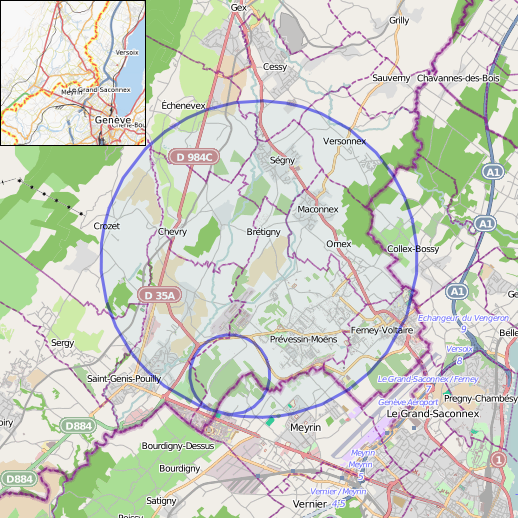
\includegraphics[width=0.5\textwidth]{figures/chapter02/Location_Large_Hadron_Collider.png}
    \bicaption{\quad \centering 大型强子对撞机(LHC)位置图~\cite{LHC}}{\quad \centering Map of the Large Hadron Collider~\cite{LHC}(LHC)}
    \label{fig:c02f01}
\end{figure}

加速器部分主要由27公里的超导磁铁环和许多加速结构构成,用于加速经过的粒子束流。在加速器内部,两束高能粒子束流可以被加速到接近光速,并且以相反的运动方向在由超导电磁体产生的强电磁场中沿着束流管道运行。超导电磁体包括了1232个偶极磁铁和392个四极磁铁。每个偶极磁铁长约15米,主要用于使粒子束流轨迹发生弯曲;每个四极磁铁长约5到7米,主要作用是聚焦束流。加速结构主要指的是射频腔,带电粒子在射频腔产生的强电场内被不断加速,通过多级加速结构,最终可以使得粒子束流的速度接近于光速的99.9999991\%。图~\ref{fig:c02f02}展示了粒子束流的加速过程:

\begin{enumerate}
    \item 通过将氢原子的核外电子剥离得到质子束流,并在直线加速器的作用下将质子束流加速到50~\si{\MeV}。
    \item 将加速后的质子束流注入到质子同步推进器中继续加速至1.4~\si{\GeV}。
    \item 继续将加速后的质子束流注入质子同步加速器中加速至25~\si{\GeV}。
    \item 质子束流被注入到超级质子同步加速器中,加速到450~\si{\GeV}。
    \item 最终,两束质子束流被分别注入到LHC的两个束流管中,以相反的方向运动,加速至7~\si{\TeV}。
\end{enumerate}

\begin{figure}[!htbp]
    \centering
    %trim option's parameter order: left bottom right top
    \includegraphics[width=1.0\textwidth]{figures/chapter02/CERN_accelerator.jpeg}
    \bicaption{\quad \centering CERN加速器综合体~\cite{accelerator}}{\quad \centering The CERN accelerator complex~\cite{accelerator}}
    \label{fig:c02f02}
\end{figure}

粒子探测器主要用于探测高能粒子发生对撞后所产生的末态粒子。根据这些产生的末态粒子,可以反推得到粒子对撞时发生的物理过程,这也是我们了解微观粒子世界的重要途径。在LHC建设之初,一共有9个探测器被建造出来,它们分别位于LHC的不同对撞点上,具有各自不同的物理实验目标,其中最主要的四个大型实验分别为ATLAS、CMS、LHCb和ALICE。ATLAS和CMS是运行在LHC上最大的两个粒子物理实验,它们都是大型的通用粒子探测器,具有相同的实验目标,包括寻找希格斯粒子、寻找额外维度以及寻找可能构成暗物质的粒子等等;LHCb探测器的主要物理目标是b物理实验,它的设计目的主要是通过测量b强子(包含一个b夸克的重粒子)的宇称不守恒来理解宇宙中的正反物质不对称性,同时它也可以对产生截面、奇特强子谱、粲物理和电弱物理进行测量;ALICE实验主要是用于研究重离子对撞(铅-铅对撞),对撞产生的高温和能量密度能够让我们对夸克-胶子等离子体进行研究,这种等离子状态被认为存在于宇宙大爆炸之后夸克和胶子结合形成强子和质量更重的粒子之前,对夸克-胶子等离子体的研究可以让我们对宇宙的起源有深刻的理解。

\section{CMS探测器简介}

CMS探测器全称紧凑型缪子线圈探测器(Compact Muon Solenoid,CMS),呈圆柱体结构,总重大约14000吨,长28.7米,直径15.0米,周围被强大的磁场所覆盖。它采用了圆柱形超导电缆线圈的形式,可以产生3.8特斯拉的超强磁场,是地球磁场的100000倍。探测器总体结构如图\ref{fig:c02f03}所示,由内向外分别为:

\begin{enumerate}
    \item 硅径迹探测器:用于测量带电粒子的运动轨迹。
    \item 晶体电磁量能器:用于测量主要通过电磁作用力相互作用的粒子的能量。
    \item 强子量能器:用于测量通过强作用力相互作用的粒子的能量。
    \item 超导螺线圈:提供强磁场,使带电粒子的运动轨迹发生弯曲,进而辨别不同质量的粒子。
    \item 缪子探测器:用于测量缪子的运动径迹。
\end{enumerate}

\begin{figure}[!htbp]
    \centering
    %trim option's parameter order: left bottom right top
    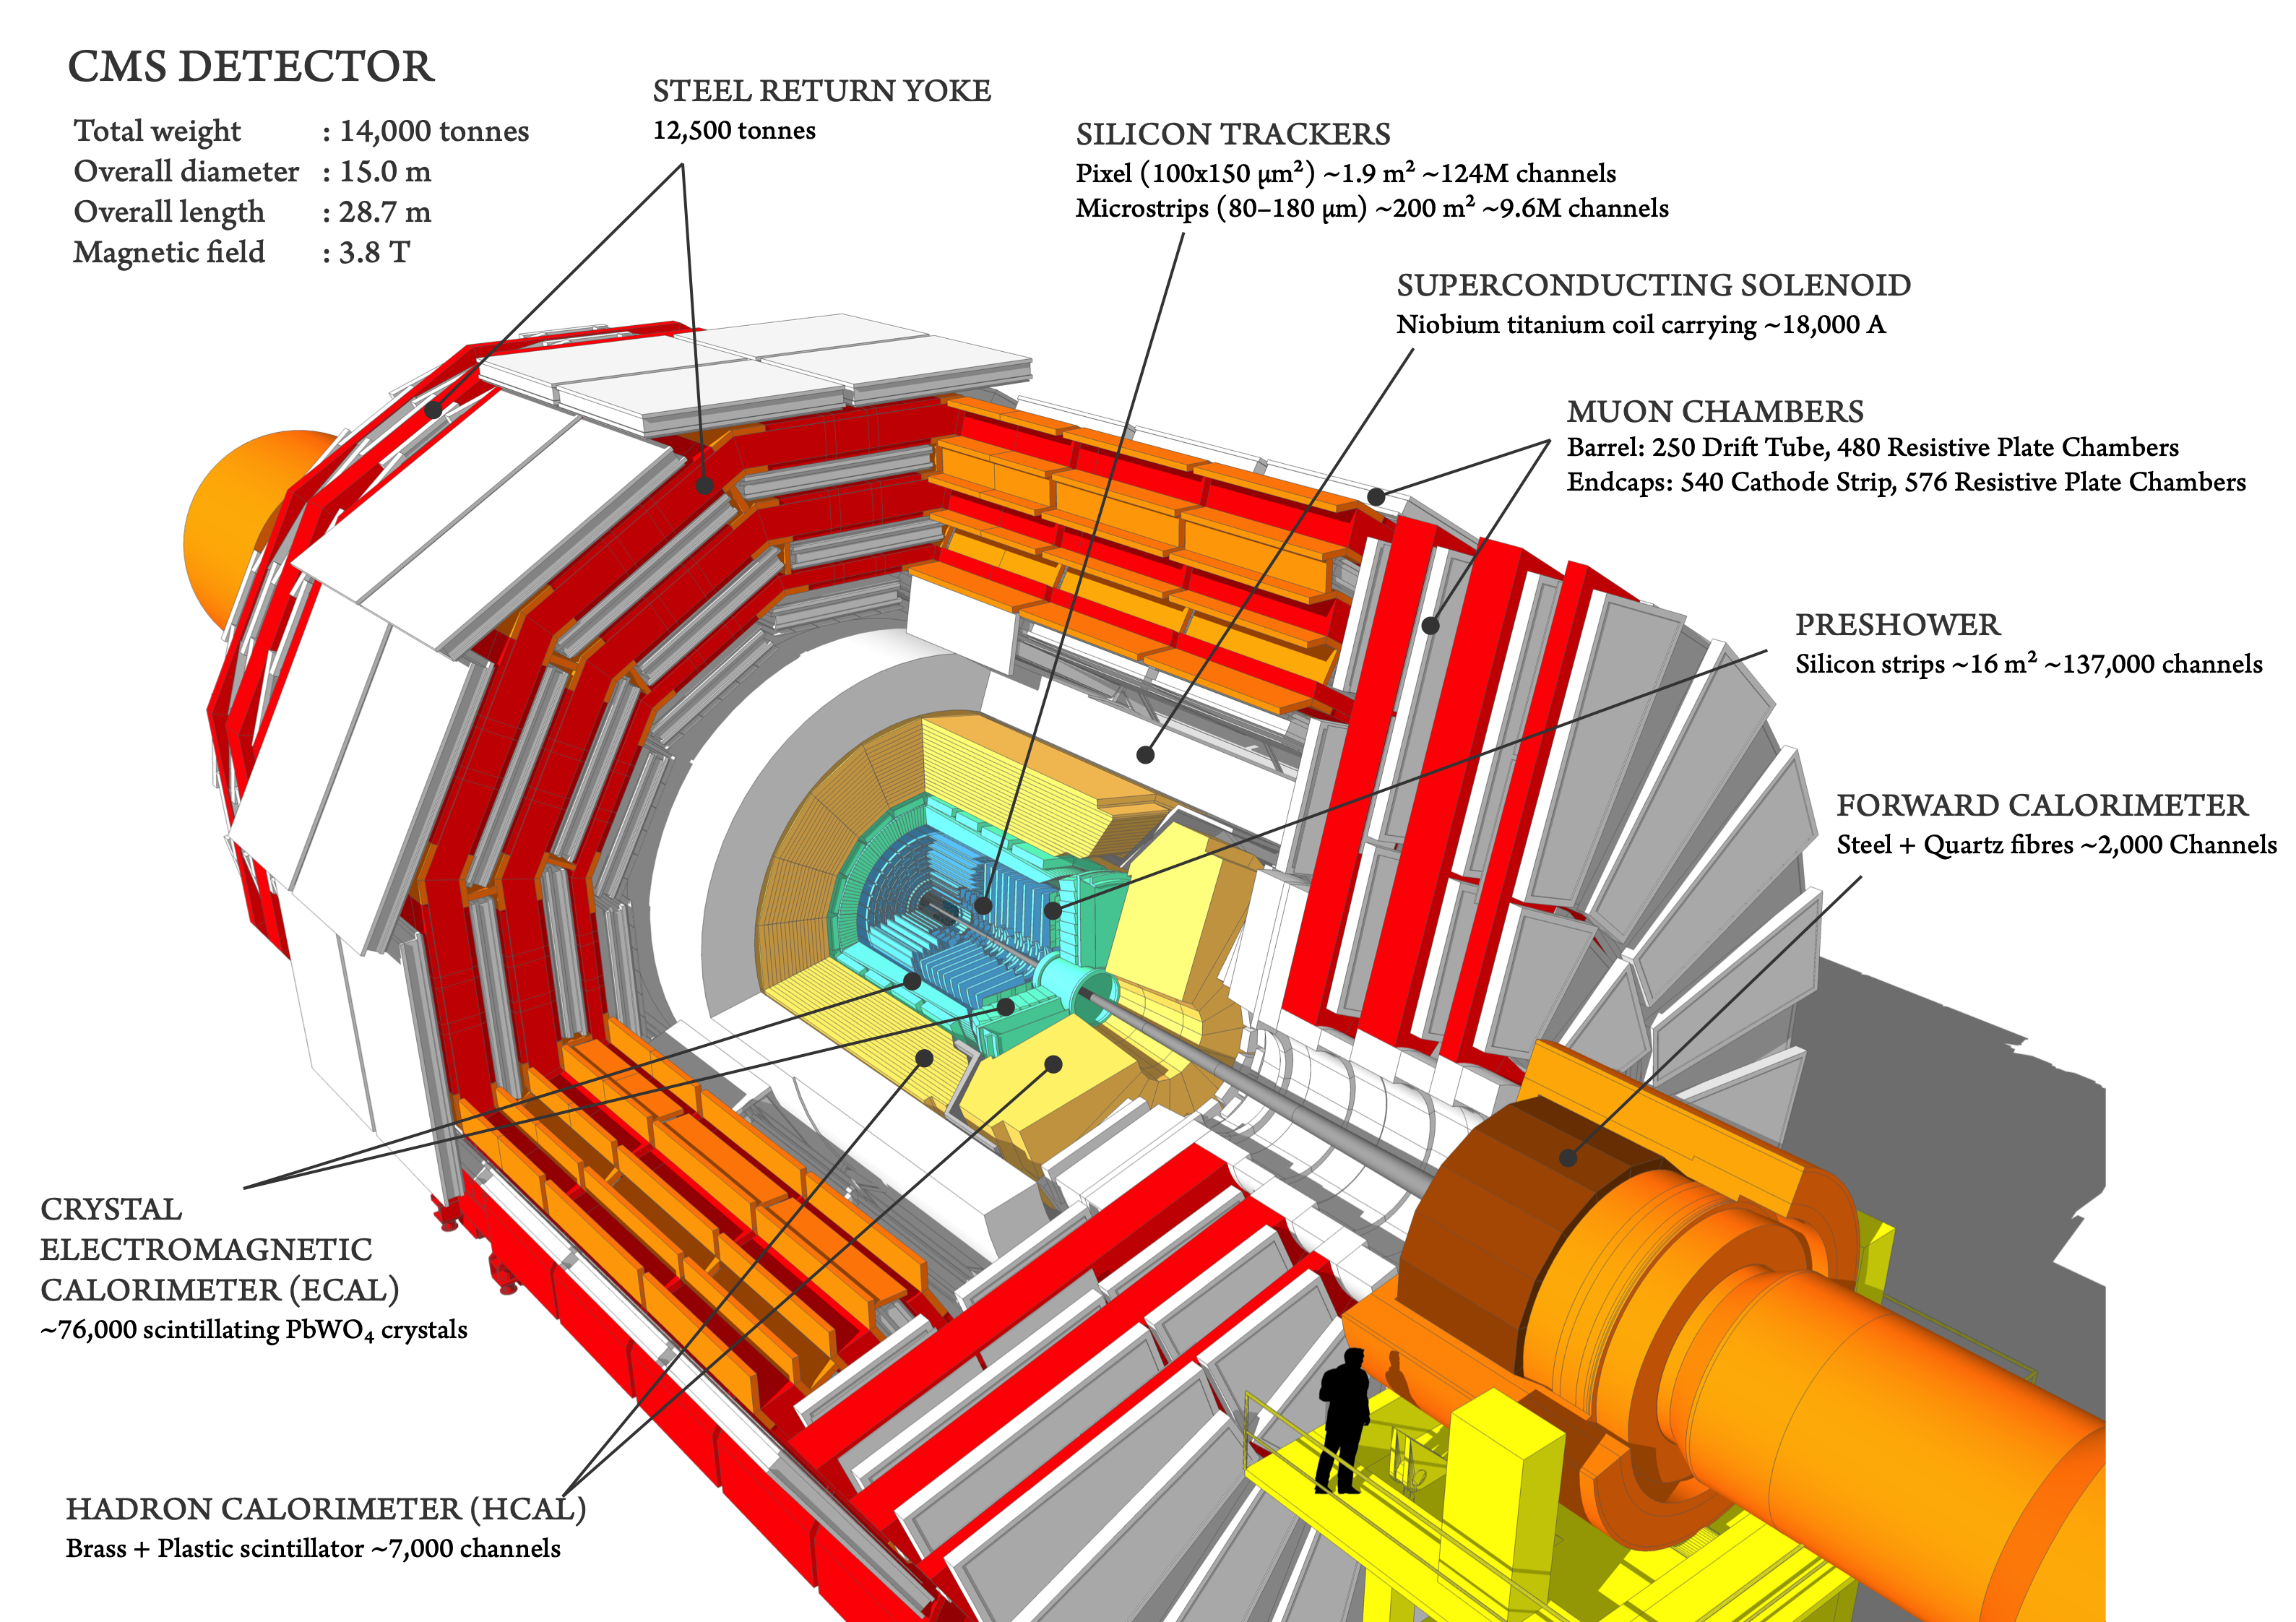
\includegraphics[width=1.0\textwidth]{figures/chapter02/CMS_160312_06.png}
    \bicaption{\quad \centering CMS探测器剖视图~\cite{Sakuma:2665537}}{\quad \centering A cutaway diagram of the CMS detector~\cite{Sakuma:2665537}}
    \label{fig:c02f03}
\end{figure}

当对撞发生时,两束在LHC环形束流管道内沿着相反方向运动的质子束流在探测器两端的磁铁作用下聚集到探测器中心并发生对撞。在完全设计的亮度下,LHC的两束质子束流都将包含2808个质子束团,其中每个质子束团都含有~\num{1.15e11}个质子,每次对撞的时间间隔为25~\si{\nano\second}。但是由于用于注射束流的磁铁在切换激活和停用的状态时存在一定时间间隔,实际的对撞次数为每秒3160万次。每次对撞平均会产生20次质子-质子相互作用,在电弱尺度下,这些散射都是由每个质子的夸克或者胶子所引发的,因此实际的对撞能量会小于束流的质心能量。在这20次的相互作用中,但绝大多数相互作用顶点都会发生弹性散射,而只有一小部分的相互作用顶点会发生非弹性散射并产生我们感兴趣的物理过程。

对撞产生的末态粒子在经过各层探测器后会被各子探测器所响应,最终重建为一个一个单独的粒子。重建出来的粒子在探测器中的位置可以用赝球面坐标系($r,\eta,\phi$)来表示,其中$r$是目标点到对撞点的距离,$\phi$是横向平面内的方位角,$\eta$是赝快度定义为$\eta = \ln{\tan{\theta/2}}$,其中$\theta$为目标点与束流方向的极角。在CMS实验中,粒子的四动量通常表述为($\pt,\eta,\phi,m$),其中$\pt$表示粒子的动量在横向的投影;$m$为粒子的质量。

在2012年CMS和ATLAS共同宣布发现希格斯粒子之后,标准模型的最后一块拼图被找到,CMS也完成了它建立之初最重要的一个物理目标。目前,CMS探测器作为一个大型通用粒子物理探测器,现在的物理目标主要有:在~\si{\TeV}级别探寻新物理;在希格斯粒子被发现后,更进一步的研究它的性质;寻找超出标准模型新物理的证据,包括超对称和额外维;研究重离子对撞。

\subsection{硅径迹探测器}

在探测器中,动量是描述一个粒子的重要信息,它对构建对撞发生时的物理过程具有至关重要的作用。由于运动的带电粒子在磁场中会受到洛伦兹力的作用,当磁场处于均匀恒定的状态时,带电粒子受到的作用力方向垂直于粒子运动方向和磁场方向。这时,带电粒子在垂直于磁场的平面上做匀速圆周运动,又称拉莫尔运动,匀速圆周运动的半径又称拉莫尔半径。根据粒子做匀速圆周运动以及受到的向心力为洛伦兹力,计算可得拉莫尔半径的表达式为:
\begin{equation}\label{eq:2-1}
    r_{g}=\frac{m v_{\perp}}{|q| B}
\end{equation}
其中,$m$为粒子质量,$v_{\perp}$为粒子垂直于磁场方向的速度,$q$是粒子的带电荷量,$B$是磁场强度。由此我们可以看出,在磁场恒定的条件下,可以通过测量粒子的回转半径(即拉莫尔半径)来计算出粒子的动量。硅径迹探测器正是通过记录带电粒子在探测器中的几个关键位置来重建出粒子轨迹,进而通过轨迹的回转半径计算出粒子的动量。

正如名称所言,CMS实验的径迹探测器完全由硅制成,包括位于探测器核心的硅像素探测器和包裹在外围的硅微条探测器,可以重建出高能缪子、电子、强子以及来自寿命非常短的粒子(比如b夸克)衰变的轨迹。由于需要精确测量粒子的位置信息同时尽可能小干扰粒子的运动轨迹,利用尽可能少的层数精确测量粒子的位置信息成为了关键。

\begin{figure}[!htbp]
    \centering
    %trim option's parameter order: left bottom right top
    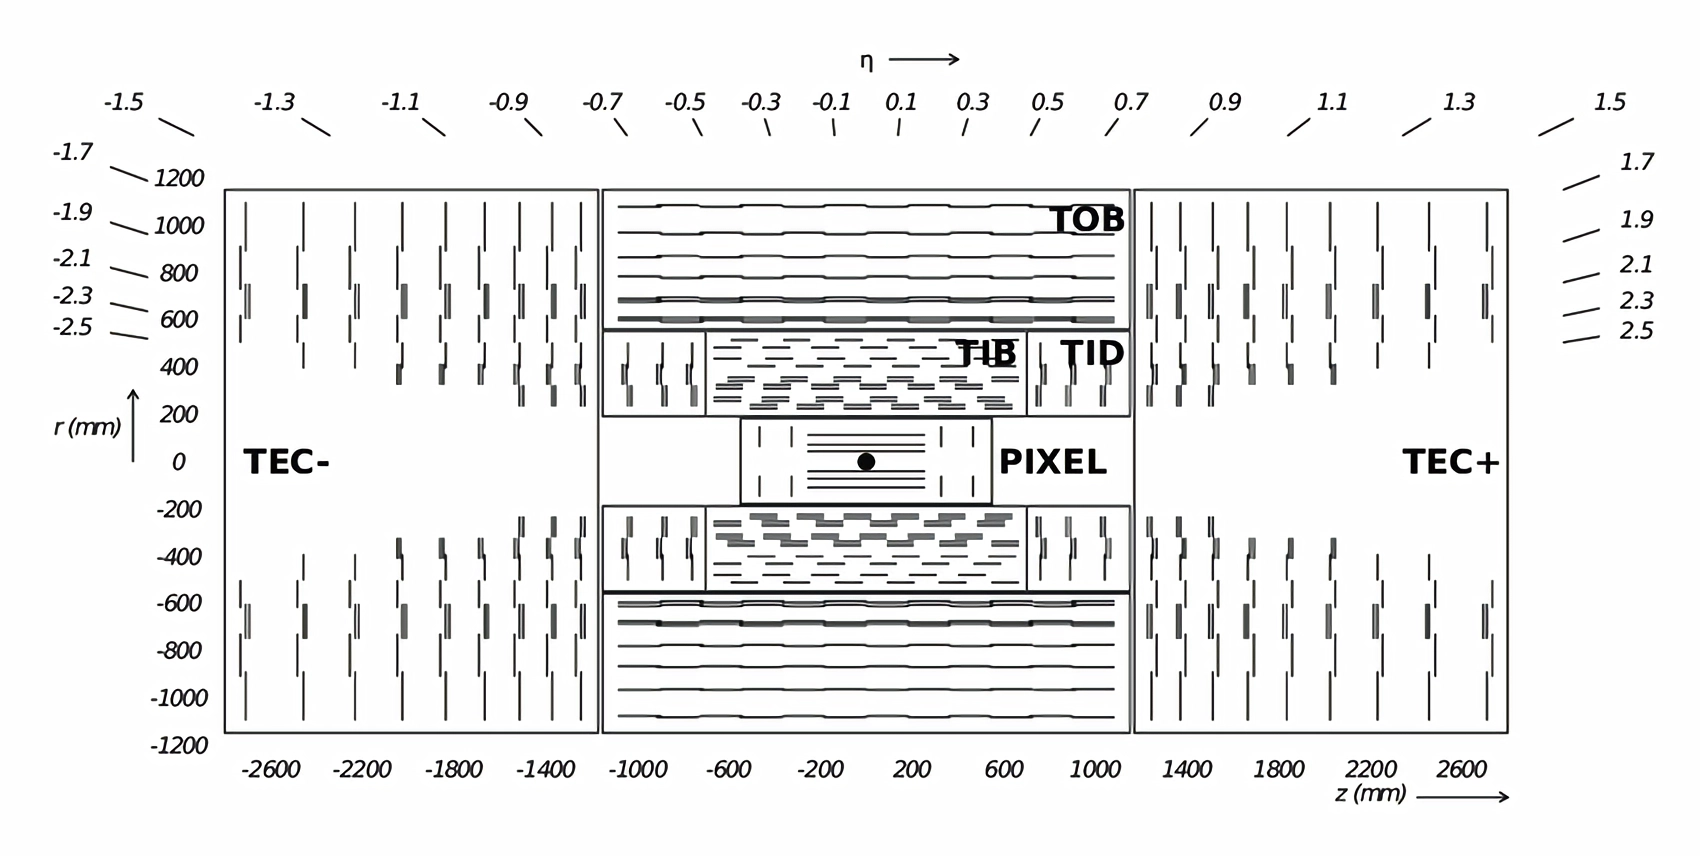
\includegraphics[width=1.0\textwidth]{Thesis (Version 2246)/figures/chapter02/Schematic-cross-section-of-the-CMS-tracker-Each-line-represents-a-detector-module.png}
    \bicaption{\quad \centering CMS径迹室示意图~\cite{Bauer:1308713}}{\quad \centering Schematic overview of the CMS tracker~\cite{Bauer:1308713}}
    \label{fig:c02f04}
\end{figure}

目前,CMS实验上的径迹探测器如图~\ref{fig:c02f04}所示,包含桶部区域的14层和端盖区域的15层探测器。它对粒子的位置测量可以精确到10~\si{\micro\meter},只有人类头发丝的十分之一。最里面的四层由100~\si{\um} $\times$ 150~\si{\micro\meter}的硅像素探测器组成,一共1.24亿个像素;剩下的均由硅微条探测器组成,包括中间四层10~\si{\centi\meter} $\times$ 180~\si{\micro\meter}的硅微条探测器以及外围六层25~\si{\centi\meter} $\times$ 180~\si{\micro\meter}的硅微条探测器,一共包含960万个硅微条探测器。当粒子经过径迹探测器时,会在探测器内部产生微弱的电信号,经过放大后的信号会被后端电子学所接收并用于粒子径迹重建。



\subsection{晶体电磁量能器}

在CMS实验中,粒子的能量对重建对撞物理过程也具有非常重要的意义。电磁量能器(ECal)的作用主要是精确测量电子和光子的能量以及沉积位置。它是由钨酸铅晶体(PbWO$_{4}$)所构成,这种物质密度非常高但是却具有光学透明性,设计目的是利用电磁簇射吸收高能粒子的能量使其沉积在探测器中并测量其能量。由于其高透明性,当电子或光子经过探测器时会使其发生闪烁,闪烁光的强度与粒子的能量成正比,通过雪崩放大后的闪烁光被后端电子学所接收并用于重建粒子的能量。选用这种材料的优势是它产生的闪烁光具有非常快的光输出,可以在一次对撞的时间内(25~\si{ns})内完成80\%的光输出。

\begin{figure}[!htbp]
    \centering
    %trim option's parameter order: left bottom right top
    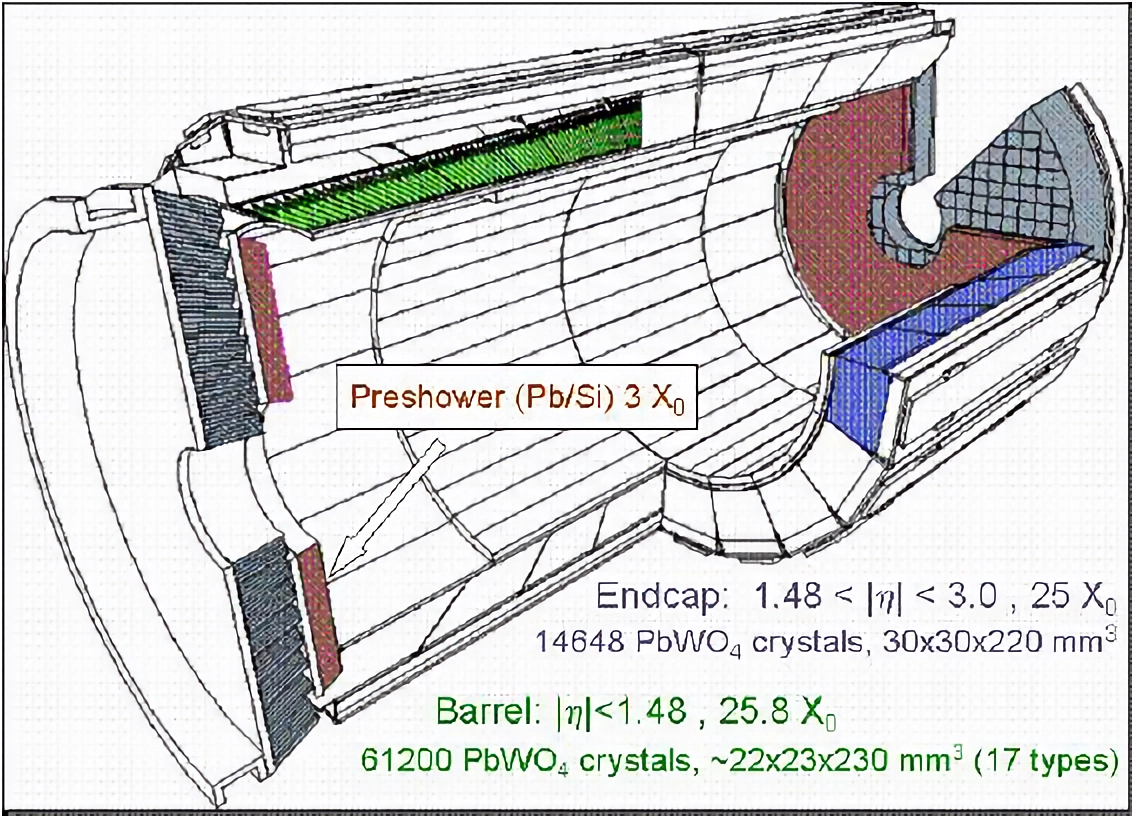
\includegraphics[width=0.8\textwidth]{figures/chapter02/View-of-the-CMS-electromagnetic-calorimeter.png}
    \bicaption{\quad \centering CMS电磁量能器外观图~\cite{ECAl}}{\quad \centering View of the CMS electromagnetic calorimeter~\cite{ECAl}}
    \label{fig:c02f05}
\end{figure}

目前在CMS实验上所使用的晶体电磁量能器的结构如图~\ref{fig:c02f05}所示 。在桶部区域,一共含有61200个晶体,每个晶体的尺寸约为22~\si{mm} $\times$ 23~\si{mm} $\times$ 230~\si{mm},构成36个超级模块;每个模块包含1700个晶体,重约三吨。端盖部分一共含有4648个晶体,尺寸为30~\si{mm} $\times$ 30~\si{mm} $\times$ 220~\si{mm}。为了增加额外的空间辨别精度,电磁量能器也包含了位于端盖前部的预簇射探测器(preshower detector),它的作用主要是探测小角度的单个高能光子或者低能光子对。

\subsection{强子量能器}

除了电子和光子的能量,重建最初对撞的物理过程也需要强子的能量信息,强子量能器(HCal)正是用于测量强子能量的探测器,其结构图如图~\ref{fig:c02f06}所示。强子量能器是由多层致密材料(黄铜或者钢)和塑料闪烁体交错组成的,这种设计的目的是为了使得磁铁线圈内的材料具有最大的能量吸收率,其中致密材料用于吸收强子的能量、塑料闪烁体用于测量粒子的能量。目前,CMS实验上的强子量能器主要有四部分:桶部部分(HB)、端盖部分(HE)、外围部分(HO)以及前向部分(HF)。

\begin{figure}[!htbp]
    \centering
    %trim option's parameter order: left bottom right top
    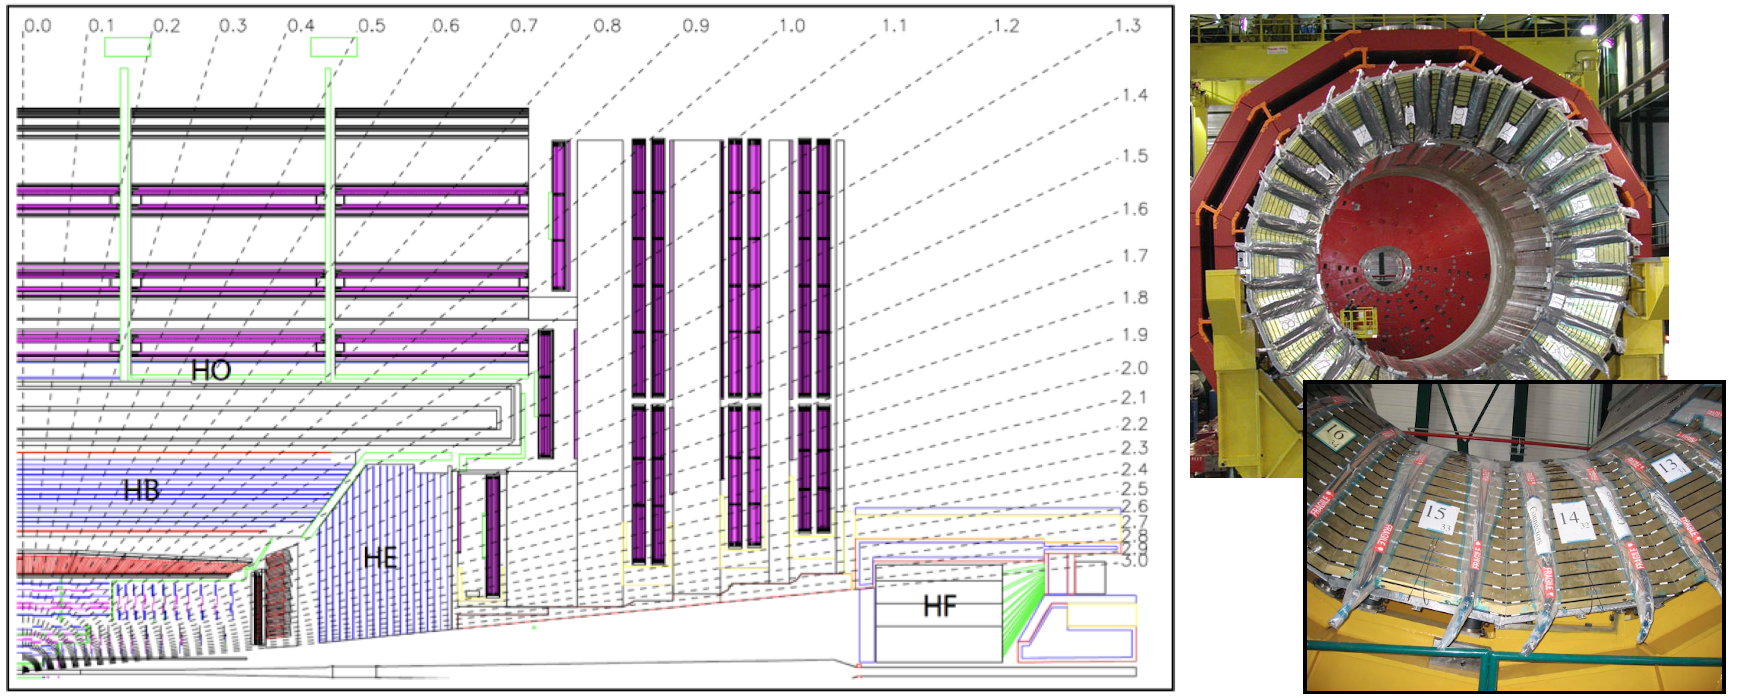
\includegraphics[width=1.0\textwidth]{figures/chapter02/hcal.png}
    \bicaption{\quad \centering CMS强子量能器示意图~\cite{phdthesis}}{\quad \centering Schematic diagram of CMS hadron calorimeter~\cite{phdthesis}}
    \label{fig:c02f06}
\end{figure}


桶部的强子量能器一共包含2304个探测器模块,每个模块所覆盖的方位角为$\Delta\eta\times\Delta\phi = 0.087\times0.087$,总共覆盖了赝快度为$-1.4<\eta<1.4$的区域。

对于端盖部分,探测器模块覆盖了赝快度为$1.3<|\eta|<3.0$的区域,总共含有2304个模块,其中最外围的5层探测器每个模块$\phi$角度覆盖范围为5\si{\degree},$\eta$角度覆盖范围为0.087;内部的8层探测器每个模块$\phi$角度覆盖范围为10\si{\degree},$\eta$角度覆盖范围为0.09到0.35。

强子量能器的外围部分主要是由10~\si{mm}厚的闪烁体探测器所构成,位于线圈外部真空罐的外围,覆盖范围为$-1.26<\eta<1.26$。它们主要的作用是对泄漏出强子量能器的强子簇射进行采样,能够在对能量分辨函数进行测量的过程中减小尾巴部分的贡献,并且提升量能器对丢失能量测量的分辨率。

强子量能器的前向部分主要覆盖了$3.0<|\eta|<5.0$的范围,与其他部分不同,前向量能器的材料由钢和石英纤维所组成。原因是强子簇射的中性部分更倾向于被前向量能器所接收,这种设计产生的强子簇射会更窄和更短,因此更适合簇射环境比较拥挤的前向部分。前向量能器位于对撞顶点11.2米处,吸收体深度为1.65米,信号来源于粒子穿过石英纤维时发出的切伦科夫光,经过光电倍增管放大后被后端电子学接收。

\subsection{磁铁系统}

CMS实验的磁铁系统如图~\ref{fig:c02f07}所示,是由一个长约12.5米、内孔直径约5.9米的超导螺线圈组成,它最大可以产生4特斯拉的超强磁场,是地球磁场的10万倍,但为了最大程度的延长磁铁的使用寿命,实际运行中产生的磁场为3.8特斯拉。这使得我们可以根据带电粒子在磁场中的弯曲轨迹来确定粒子的荷质比,进而来辨别粒子种类。

\begin{figure}[!htbp]
    \centering
    %trim option's parameter order: left bottom right top
    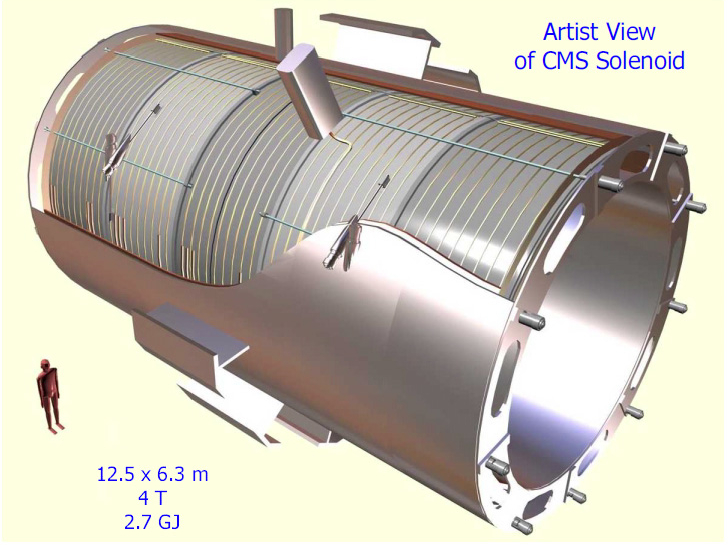
\includegraphics[width=0.8\textwidth]{figures/chapter02/CMS-solenoid-magnet.jpeg}
    \bicaption{\quad \centering CMS螺线管磁铁~\cite{Magnet}}{\quad \centering CMS solenoid magnet~\cite{Magnet}}
    \label{fig:c02f07}
\end{figure}

径迹室、电磁量能器和强子量能器都位于螺线管内部,缪子探测器围绕着螺线管排布在外围。与此同时,巨大的磁铁也为整个实验提供了绝大多数的结构支撑。

\subsection{缪子探测器}\label{sec:MuonDetector}

正如CMS实验的名称“紧凑型缪子探测器”所提到的,探测缪子是CMS实验中最重要的目标之一。在希格斯粒子的研究中,四个缪子末态对精确测量希格斯粒子的质量和宽度起到了至关重要的作用。缪子探测器的主要目标是通过记录缪子的飞行轨迹来测量缪子的动量。

缪子是带电粒子,电荷量和电子相同,但是质量却是电子的200倍。不像其他粒子会被量能器所吸收,缪子和其他物质的相互作用非常微弱,通常可以穿过整个探测器到达探测器外围甚至飞出整个探测器。因此,缪子探测器被摆放在整个CMS探测器最外围,只有缪子是唯一可能产生信号的来源。

\begin{figure}[!htbp]
    \centering
    %trim option's parameter order: left bottom right top
    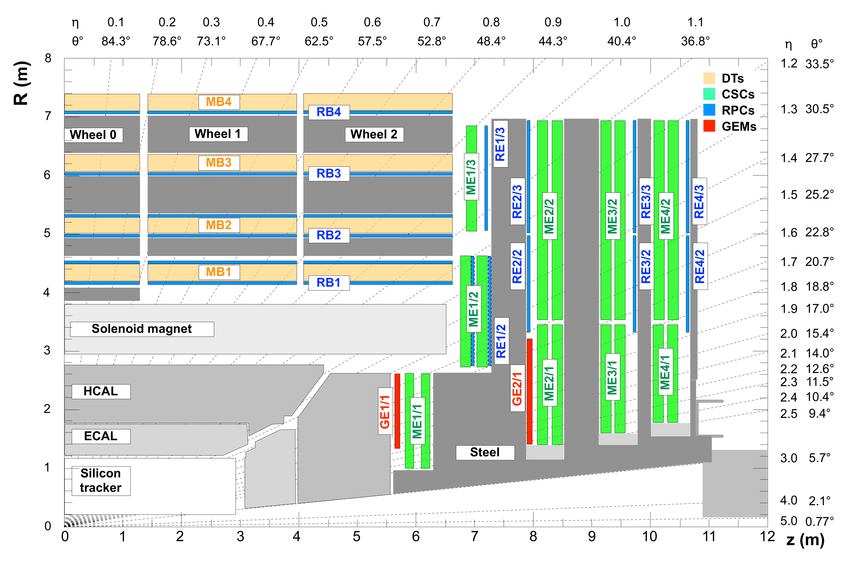
\includegraphics[width=0.8\textwidth]{figures/chapter02/Quadrant-of-the-CMS-detector-showing-the-present-muon-system-including-RPCs-DTs-and.png}
    \bicaption{\quad \centering CMS缪子系统~\cite{MuonSystem}}{\quad \centering CMS Muon system~\cite{MuonSystem}}
    \label{fig:c02f08}
\end{figure}

目前运行在CMS实验上的缪子探测器如图~\ref{fig:c02f08}所示,主要由四部分探测器所组成:漂移管道室(DT)、阴极条形室(CSC)、电阻板室(RPC)和气体电子倍增器(GEM)。DT用于精确测量桶部的缪子轨迹;而CSC用于端盖的缪子轨迹测量;RPC可以在缪子通过探测器时提供快速的信号响应,因此同时被安装在了桶部和端盖。这四种探测器都属于气体探测器,密闭的空间中充入介质气体,并且包含一个阳极面和阴极面。当缪子或者任何带电粒子经过探测器时,会使气体发生电离并将气体中原子的核外电子剥落,这些电子会随着电场的方向漂移到阳极丝,阳离子会漂向阴极板,最终被前端电子学所收集成为信号。

漂移管道室(Drift Tube chamber, DT)的结构如图~\ref{fig:c02f09}所示,它是一种气体漂移室,每根4厘米宽的气体管子中间包含有一根拉伸的金属丝,气体介质为Ar和CO$_2$的混合气体。每个漂移管道室的平均尺寸为2~\si{m} $\times$ 2.5~\si{m},由12层铝层构成,分为三组,每组四个,每层最多由60个漂移管道所构成;三组中中间一组测量平行于束流方向的坐标,另外两组测量垂直于束流方向的坐标。

\begin{figure}[!htbp]
    \centering
    %trim option's parameter order: left bottom right top
    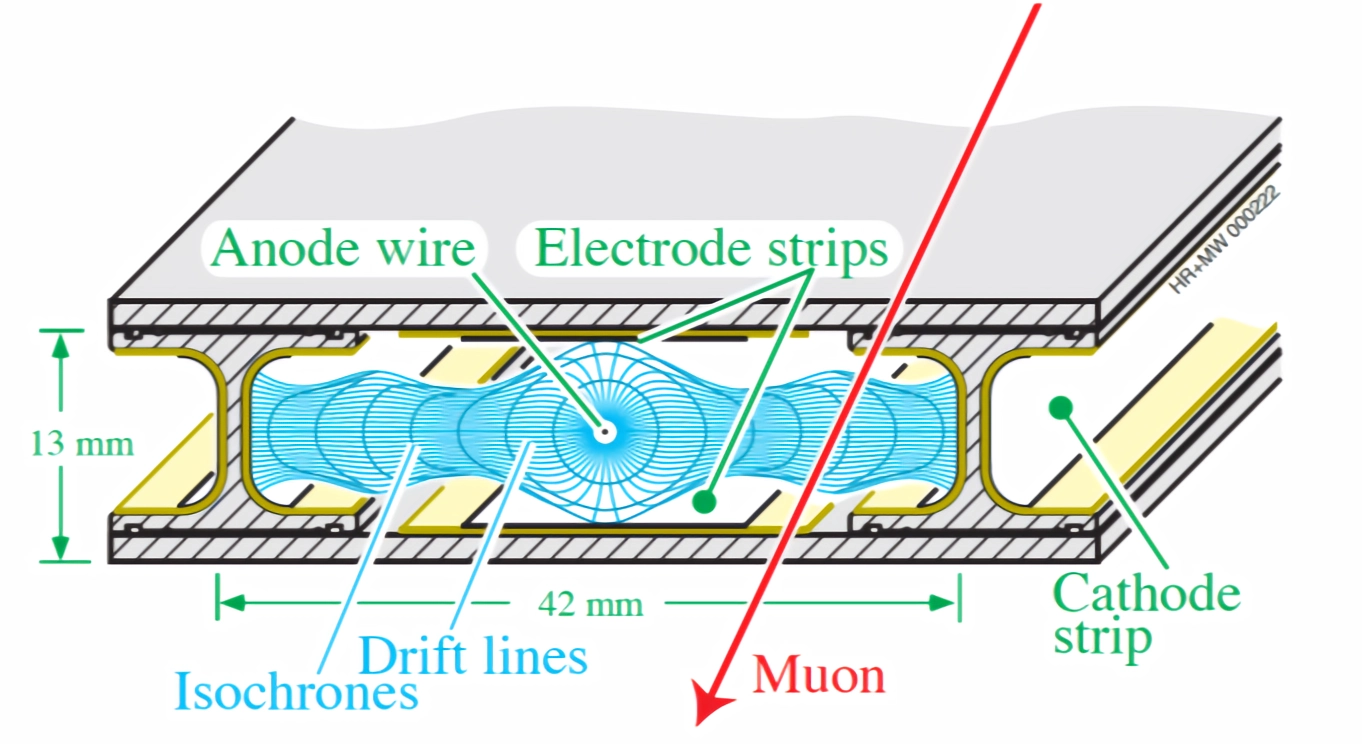
\includegraphics[width=1.0\textwidth]{Thesis (Version 2246)/figures/chapter02/DT.png}
    \bicaption{\quad \centering DT探测器示意图~\cite{Guiducci:1027479}}{\quad \centering Schematic view of the DT detector~\cite{Guiducci:1027479}}
    \label{fig:c02f09}
\end{figure}

阴极条形室(Cathode strip chambers, CSC)的结构如图~\ref{fig:c02f10}所示,每个探测器由六层宽度为9.5~\si{mm}的气体漂移室组成,每层都是由位于中间的阳极丝和位于两边的阴极条形板所组成,它们呈垂直方向。每根阳极丝之间的距离为3.12\si{mm},每根阴极条之间相距3.16~\si{mm},气体由50\%的CO$_2$、40\%的Ar和10\%的CF$_4$混合组成。当缪子穿过探测器时,会使探测器中的气体分子发生电离,在外置电场的作用下,电离产生的电子被雪崩放大,最终运动到阳极丝附近被吸收,使得阳极前端板(Anode Front End Board, AFEB)接收到信号;与此同时,电离产生的阳离子在电场的作用下漂移到阴极板,使得阴极前端板(Cathode Front End Board, CFEB)接收到信号。将AFEB和CFEB中的信号进行配对匹配,就可以确认是否信号真正来源于缪子所产生的击中。目前CMS实验上两个端盖部分的CSC探测器均由四个大圆形环所构成,一共有540个阴极条形室。由于阳极丝和阴极条形板之间互相垂直,CSC探测器可以测量粒子的二维坐标;此外,由于紧密排列的电线使得CSC探测器能够快速的探测粒子经过的信号,这使得CSC探测器也成为了触发系统的一部分。

\begin{figure}[!htbp]
    \centering
    %trim option's parameter order: left bottom right top
    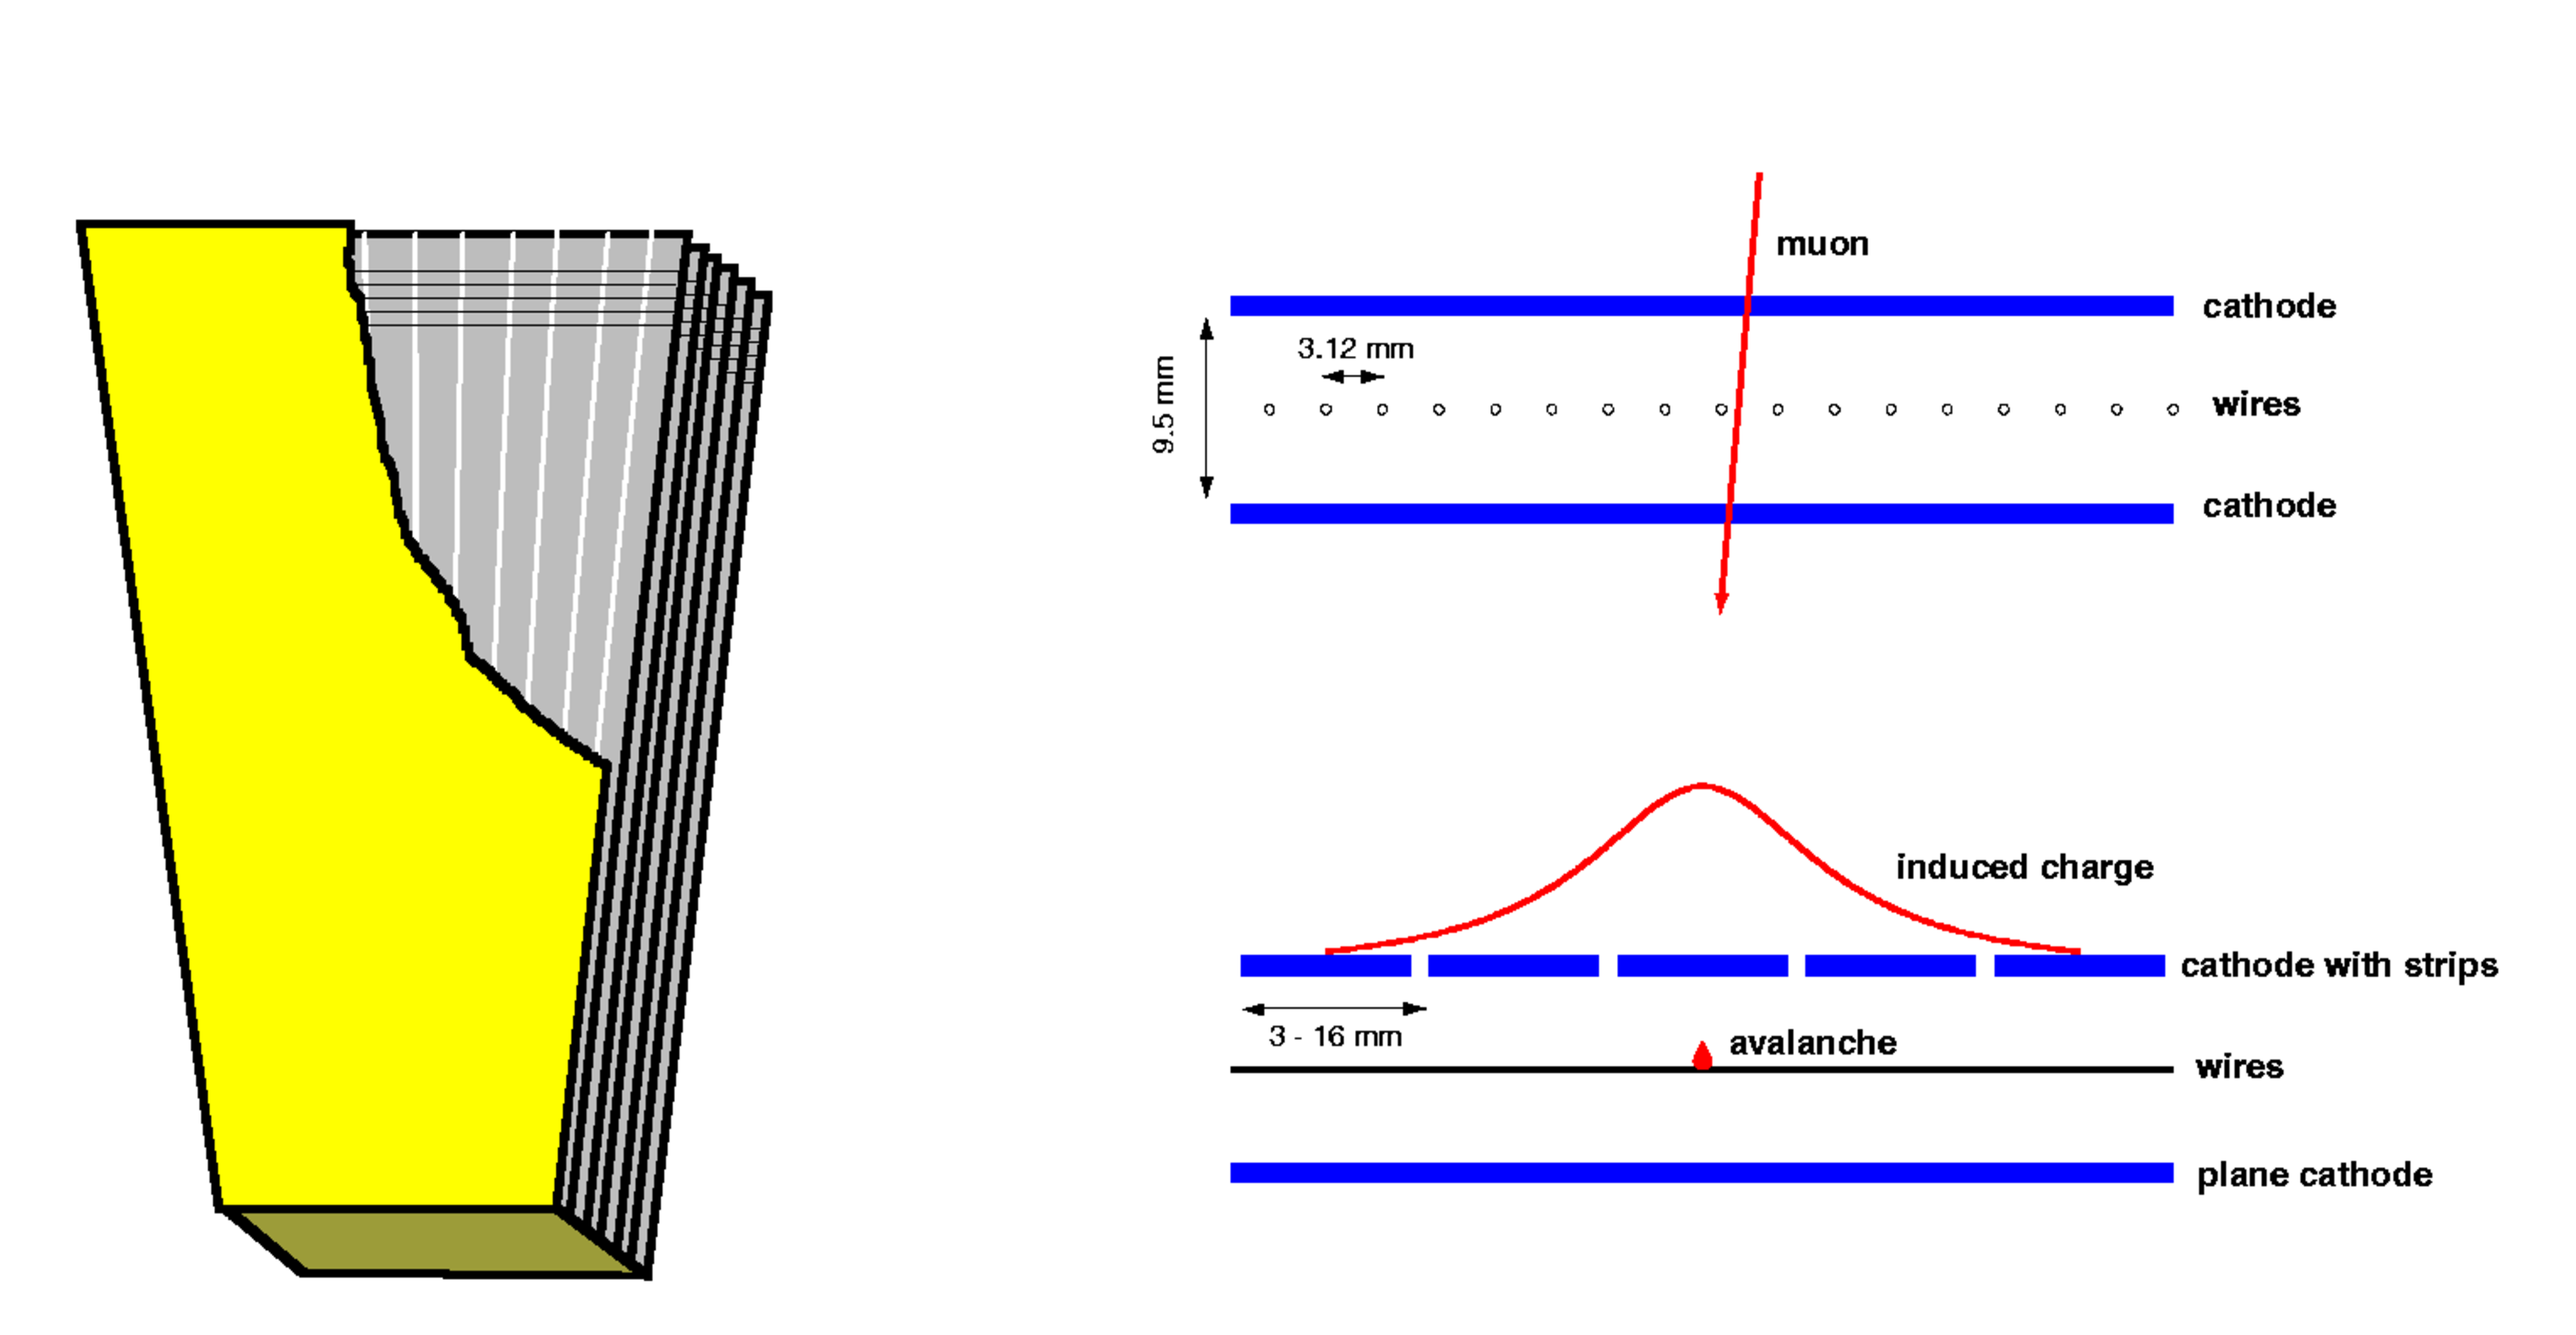
\includegraphics[width=0.8\textwidth]{Thesis (Version 2246)/figures/chapter02/CSC.pdf}
    \bicaption{\quad \centering CSC探测器示意图~\cite{CSC}}{\quad \centering Schematic view of the CSC detector~\cite{CSC}}
    \label{fig:c02f10}
\end{figure}

电阻板室(Resistive plate chambers, RPC)的结构如图~\ref{fig:c02f11}所示,它由两个平行的平面所构成,一个是带正电的阳极板,另一个是带负电的阴极条形板,它们都是由电阻率非常高的塑料材料所制成,中间用气体隔开。RPC探测器具有非常好的空间辨别率以及仅为1~\si{ns}的时间分辨率,使得它可以作为与DT和CSC探测器互相平行的缪子触发系统。

\begin{figure}[!htbp]
    \centering
    %trim option's parameter order: left bottom right top
    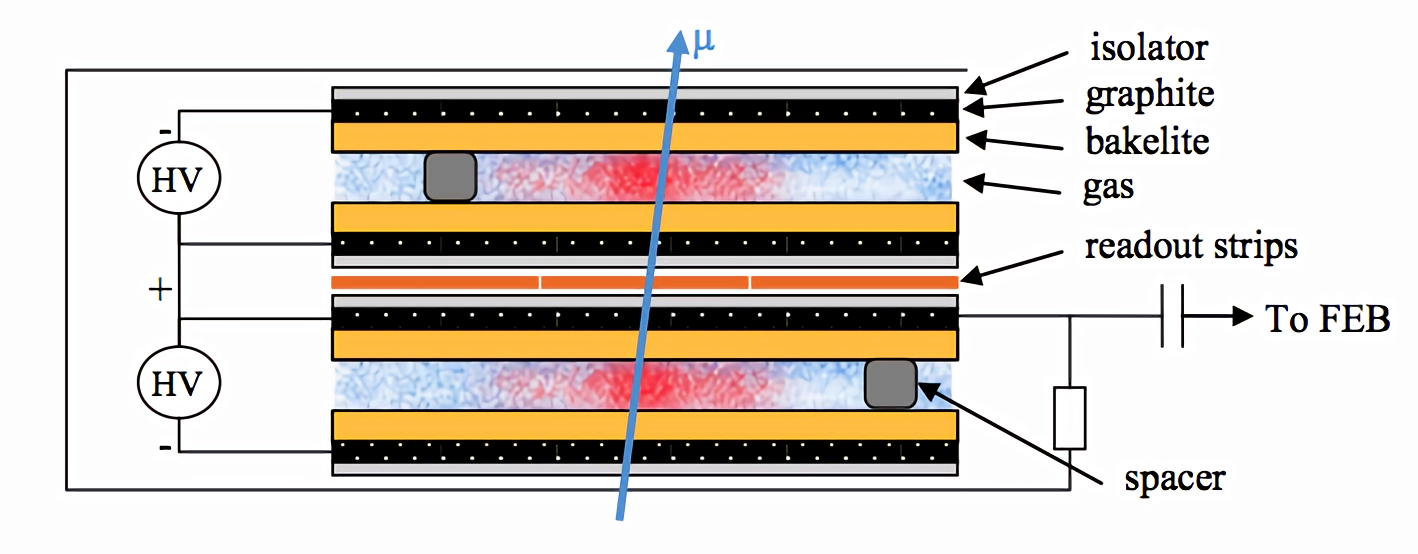
\includegraphics[width=1.0\textwidth]{figures/chapter02/rpc-schema.png}
    \bicaption{\quad \centering RPC探测器示意图~\cite{RPC}}{\quad \centering Schematic view of the RPC detector~\cite{RPC}}
    \label{fig:c02f11}
\end{figure}

气体电子倍增器(Gas electron multiplier, GEM)是运行在CMS实验上新的缪子探测系统,它们是LHC在2阶段停机升级期间安装完成的,主要目的是补充端盖现有的缪子探测系统。由于端盖区域是CMS探测器受到辐射最大和事例率最高的区域,GEM探测器可以提供额外的测量点,从而可以获得更好的缪子径迹辨别以及更大范围的端盖覆盖区域。GEM探测器的结构如图~\ref{fig:c02f12}所示,它是由三层50~\si{um}厚的覆铜聚酰亚胺箔所构成,中间充满了Ar和CO$_2$的混合气体。

\begin{figure}[!htbp]
    \centering
    %trim option's parameter order: left bottom right top
    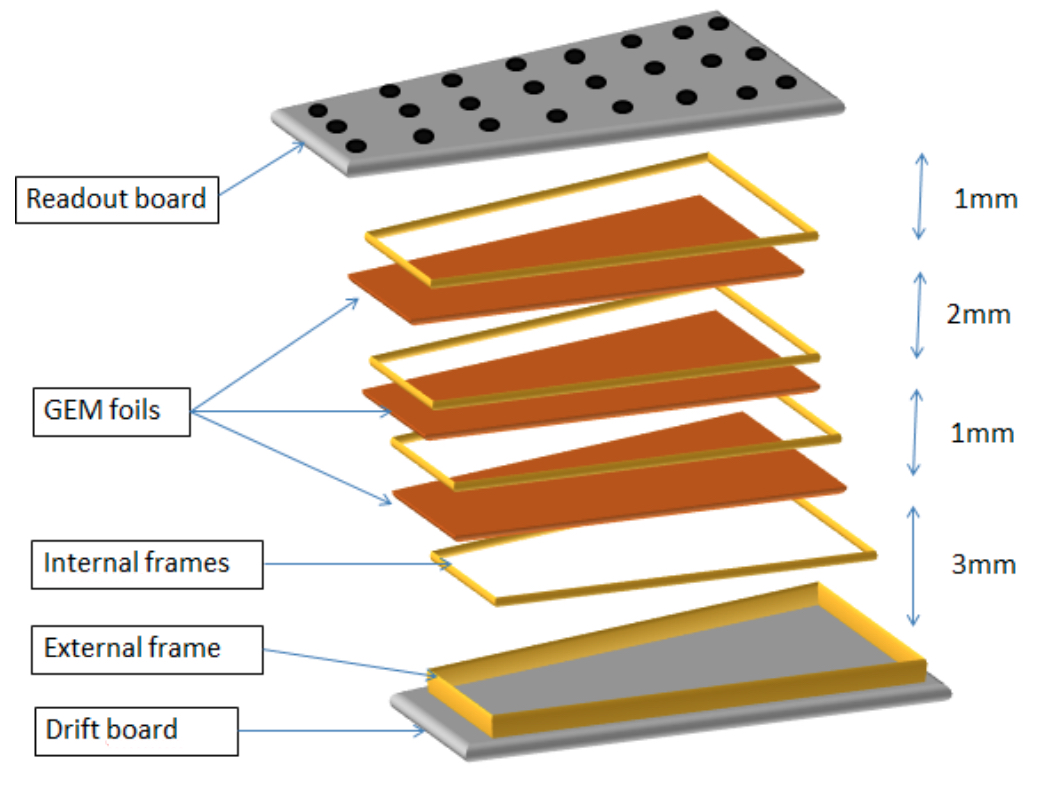
\includegraphics[width=0.6\textwidth]{figures/chapter02/GEM.jpg}
    \bicaption{\quad \centering GEM探测器示意图~\cite{CALABRIA20161042}}{\quad \centering Schematic view of the GEM detector~\cite{CALABRIA20161042}}
    \label{fig:c02f12}
\end{figure}

\subsection{触发以及数据获取}

在CMS实验中,束流对撞频率为25~\si{ns}一次,40~\si{MHz},平均每次对撞产生的原始数据量为1~MB,这就意味着每秒钟在CSM探测器中可以产生40~\si{TB}的原始数据,而这其中的绝大多数事例都是我们所不感兴趣的弹性碰撞。如此庞大的数据量不可能同时都被存储系统所记录下来,因此触发系统的作用就是尽可能快速的利用部分原始信息只过滤出我们感兴趣的事例。为了完成这个目标,在CMS实验中采用了多级触发的形式,完整的触发系统可以将每秒钟记录的事例数控制在1000个。图~\ref{fig:c02f13}展示了CMS实验的触发系统,主要由两部分构成:一级触发(Level 1 trigger)和高级触发(High Level trigger)。

\begin{figure}[!htbp]
    \centering
    %trim option's parameter order: left bottom right top
    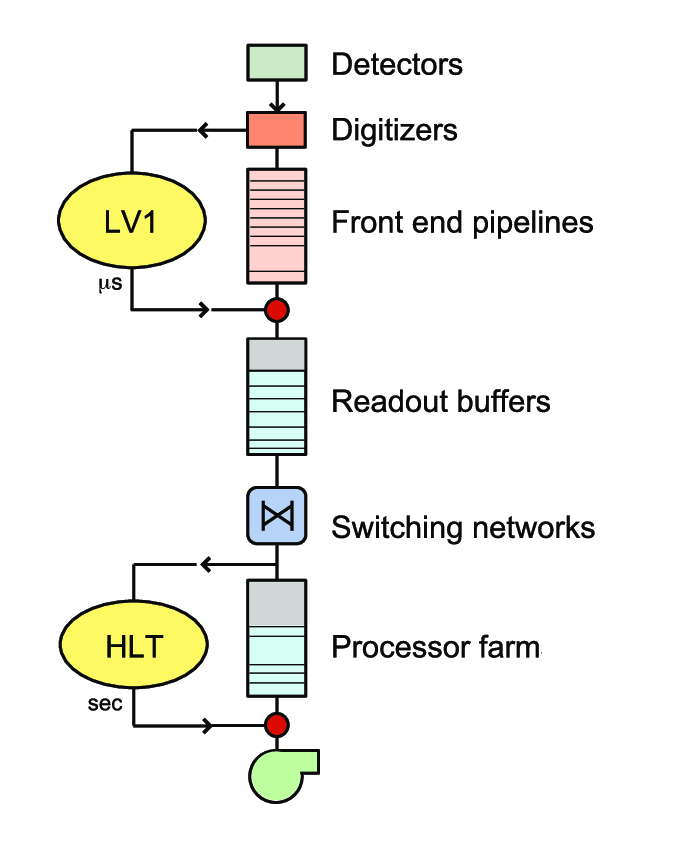
\includegraphics[width=0.6\textwidth]{figures/chapter02/trigger.png}
    \bicaption{\quad \centering CMS触发系统示意图~\cite{trigger}}{\quad \centering Schematic view of the CMS trigger system~\cite{trigger}}
    \label{fig:c02f13}
\end{figure}

对于一级触发,每次对撞的所有信息都被存储在探测器的缓存中,只有少量的关键信息被用于执行快速的、近似的计算,并用于识别我们感兴趣的特征,比如说:高能喷注、缪子或者丢失的能量。这个计算可以在大约1~\si{ns}的时间内完成,并且可以将每秒钟总的事例数降低大约1000倍,达到50~\si{kHz}。所有的这些计算都是基于硬件来完成的,因此一级触发也称为硬件触发。

对于通过一级触发的事例,缓存在探测器中的对撞数据将通过光纤链路传递给高级触发。高级触发通常指的是运行在计算机服务器上的软件,因此也称为软件触发。由于经过一级触发后到达高级触发的事例数发生了明显降低,这就使得高级触发有足够多的时间进行更加详细的分析。最终,通过高级触发的事例数可以再降低100倍,达到每秒钟1000个事例,这些事例作为我们感兴趣的事例最终被存储到磁带上并用于之后的物理分析。